\documentclass{report}

% Packages
\usepackage[utf8]{inputenc}
\usepackage[spanish]{babel}
\usepackage{amsmath}
\usepackage{amssymb}
\usepackage{amsthm}
\usepackage{graphicx}
\usepackage{float}
\usepackage{listings}
\usepackage{hyperref}
\usepackage[square,sort,comma,numbers]{natbib}
\usepackage{url}
% All in preamble:

\usepackage{listings}
\usepackage{courier}
\usepackage{color}

\definecolor{mygreen}{rgb}{0,0.6,0}
\definecolor{mygray}{rgb}{0.5,0.5,0.5}
\definecolor{mymauve}{rgb}{0.58,0,0.82}
\lstset{ %
  backgroundcolor=\color{white},   % choose the background color; you must add \usepackage{color} or \usepackage{xcolor}
  basicstyle=\footnotesize\ttfamily,        % the size of the fonts that are used for the code
  breakatwhitespace=false,         % sets if automatic breaks should only happen at whitespace
  breaklines=true,                 % sets automatic line breaking
  captionpos=b,                    % sets the caption-position to bottom
  commentstyle=\color{mygreen},    % comment style
  deletekeywords={...},            % if you want to delete keywords from the given language
  escapeinside={\%*}{*)},          % if you want to add LaTeX within your code
  extendedchars=true,              % lets you use non-ASCII characters; for 8-bits encodings only, does not work with UTF-8
  frame=single,                    % adds a frame around the code
  keepspaces=true,                 % keeps spaces in text, useful for keeping indentation of code (possibly needs columns=flexible)
  keywordstyle=\color{blue},       % keyword style
  language=Python,                 % the language of the code
  otherkeywords={*,...},            % if you want to add more keywords to the set
  numbers=left,                    % where to put the line-numbers; possible values are (none, left, right)
  numbersep=5pt,                   % how far the line-numbers are from the code
  numberstyle=\tiny\color{mygray}, % the style that is used for the line-numbers
  rulecolor=\color{black},         % if not set, the frame-color may be changed on line-breaks within not-black text (e.g. comments (green here))
  showspaces=false,                % show spaces everywhere adding particular underscores; it overrides 'showstringspaces'
  showstringspaces=false,          % underline spaces within strings only
  showtabs=false,                  % show tabs within strings adding particular underscores
  stepnumber=2,                    % the step between two line-numbers. If it's 1, each line will be numbered
  stringstyle=\color{mymauve},     % string literal style
  tabsize=2,                       % sets default tabsize to 2 spaces
  title=\lstname                   % show the filename of files included with \lstinputlisting; also try caption instead of title
}

\hypersetup{
    colorlinks=true,
    linkcolor=blue,
    filecolor=magenta,      
    urlcolor=cyan,
    pdftitle={Overleaf Example},
    pdfpagemode=FullScreen,
}

\theoremstyle{definition}
\newtheorem{definition}{Definición}[section]


\begin{document}

\begin{titlepage}
    \begin{center}
        \vspace*{1cm}
 
        \Large\textbf{Fractales}
 
        \vspace{0.5cm}
         Ejemplos, historia y aplicaciones
             
        \vspace{1.5cm}
 
        \textbf{Antonio Cabrera y Alejandro Gómez}
 
        \vfill
             
        Trabajo para el doble grado de\\
        Ingeniería del Software y Matemática Computacional\\
             
        \vspace{0.8cm}
      
        
\includegraphics[width=0.4\textwidth]{figures/logo u-tad.png}
             
        Asignatura de topología\\
        U-tad\\
        España\\
        Noviembre 2023
             
    \end{center}
 \end{titlepage}

\tableofcontents

\listoffigures

\chapter{Introducción}

\section{¿Qué es un fractal?}

La definición más inmediata que tenemos de los fractales es la siguiente:

\begin{definition}
    Un fractal es un objeto geométrico cuya estructura básica, fragmentada o irregular, se repite a diferentes escalas.
\end{definition}

\noindent Que su estructura básica se repita a diferentes escalas significa que el objeto es autosimilar.

\section{Autosimilitud}

Benoît Mandelbrot la definió como sigue:

\begin{definition}
    Un objeto es autosimilar o autosemejante si sus partes tienen la misma forma o estructura que el todo, aunque pueden presentarse a diferente escala y pueden estar ligeramente deformadas.
\end{definition}

\noindent
\large Vamos a ver dos tipos de autosimilitud:

\subsection{Autosimilitud exacta}

\begin{definition}
    Un objeto es exactamente autosimilar si es exactamente igual a sí mismo a diferentes escalas..
\end{definition}

\noindent
Es la más restrictiva de todas y la que vemos en los fractales clásicos. Algunos ejemplos de objetos exactamente autosimilares son:

\begin{itemize}
    \item El triángulo de Sierpinski
    
    \begin{figure}[H]
        \centering
        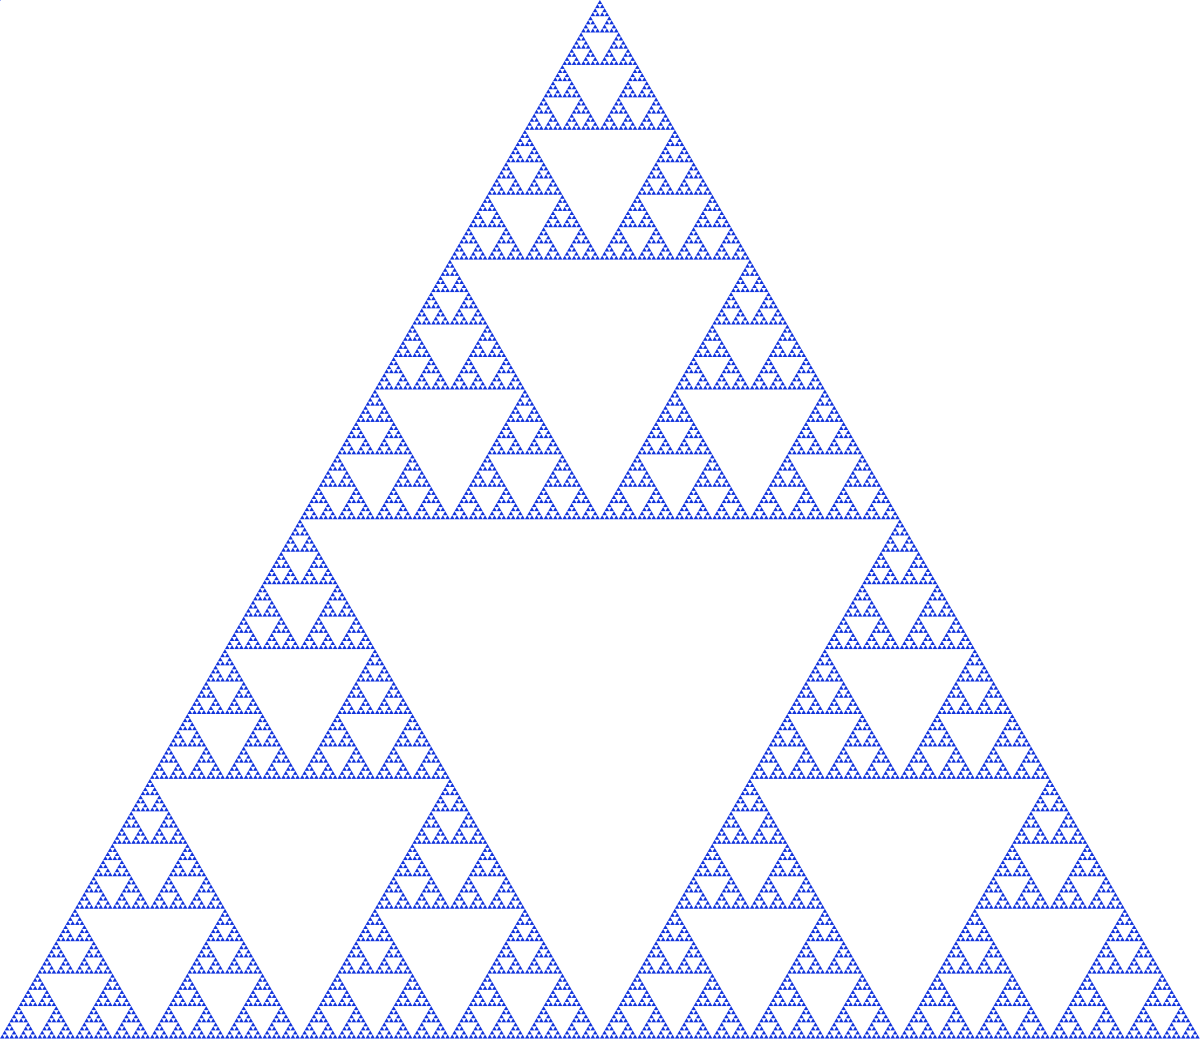
\includegraphics[width=0.5\textwidth]{figures/sierpinski-triangle.png}
        \caption{Triángulo de Sierpinski}
    \end{figure}

    \item El copo de Koch
    
    \begin{figure}[H]
        \centering
        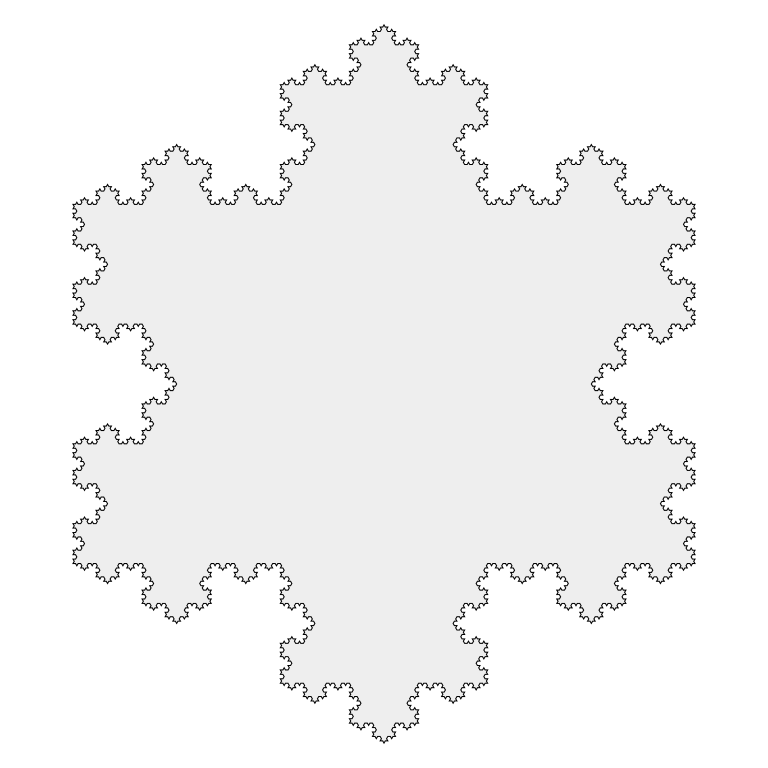
\includegraphics[width=0.5\textwidth]{figures/koch-snowflake.png}
        \caption{Copo de Koch}
    \end{figure}

\end{itemize}

\subsection{Cuasiautosimilitud}

\begin{definition}
    Un objeto es cuasiautosimilar si es aproximadamente igual a sí mismo a diferentes escalas.
\end{definition}

\noindent
Los fractales de este tipo contienen copias menores y distorsionadas de si mismos, como occure por ejemplo con el conjunto de Mandelbrot.

\begin{figure}[H]
    \centering
    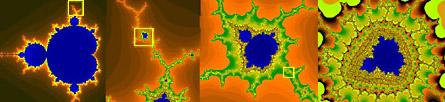
\includegraphics[width=0.7\textwidth]{figures/mandelbrot-cuasi.png}
    \caption{Ejemplos de cuasiautosimilitud en el conjunto de Mandelbrot}
\end{figure}


\section{Definición más formal}

\noindent En 1982 Benoît Mandelbrot definió los fractales de la siguiente forma:

\begin{definition}
Un fractal es un conjunto cuya dimensión de Hausdorff-Besicovitch es estrictamente mayor que su dimensión topológica.
\end{definition}

\noindent La dimensión topológica es la dimensión que todos conocemos, la dimensión de Hausdorff-Besicovitch es una de las formas de calcular la dimensión fractal de un objeto. 

\section{Dimensión fractal}

\noindent La dimensión fractal es una medida de la complejidad de un objeto fractal. La dimensión topológica de un objeto es un número entero, mientras que la dimensión fractal es un número real. La dimensión fractal es una generalización de la dimensión topológica.

\subsection{Cálculo de la dimensión fractal}

\noindent Ya hemos visto que una de las formas de calcular la dimensión fractal de un objeto es la dimensión de Hausdorff-Besicovitch, sin embargo esta resulta algo compleja. Otra forma más sencilla es con el método de \textit{Box Counting} también llamado o también conocido como la dimensión de Minkowski-Bouligard.\\

\noindent Para entender mejor este método vamos a verlo con un ejemplo. Consideremos un segemento y el borde de un cuadrado ambos de lado $1$.

\begin{figure}[H]
    \centering
    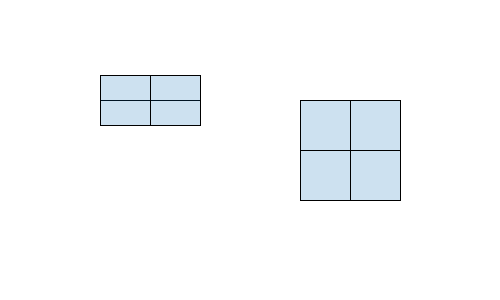
\includegraphics[width=0.7\textwidth]{figures/boxcounting-1.png}
    \caption{Box Counting - Cajas de lado $\frac{1}{2}$}
\end{figure}

\noindent Si intentamos cubrir ambos objetos con cajas de lado $\frac{1}{2}$ vemos que para el segmento necesitamos $2$ y para el cuadrado $2^2$

\begin{figure}[H]
    \centering
    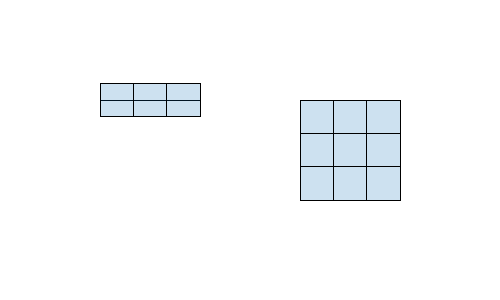
\includegraphics[width=0.7\textwidth]{figures/boxcounting-2.png}
    \caption{Box Counting - Cajas de lado $\frac{1}{3}$}
\end{figure}

\noindent Si utilizamos cajas más pequeñas, de lado $\frac{1}{3}$, vemos que para el segmento necesitamos $3$ y para el cuadrado $3^4$

\begin{figure}[H]
    \centering
    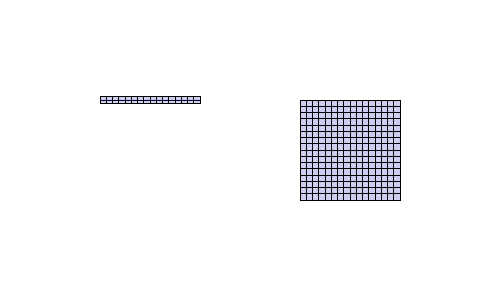
\includegraphics[width=0.7\textwidth]{figures/boxcounting-3.png}
    \caption{Box Counting - Cajas de lado $\frac{1}{n}$}
\end{figure}

\noindent Si continuamos con este proceso vemos que para el segmento necesitamos $n$ cajas de lado $\frac{1}{n}$ y para el cuadrado $n^2$\\

\noindent Vemos que el exponente es un buen indicador de la dimensión de los objetos. Si definimos $N(n)$ como el número de cajas de lado $\frac{1}{n}$ necesarias para cubrir el objeto, entonces tenemos que:

\begin{equation}
    N(n) = n^d
\end{equation}

\noindent Sacando logaritmos a ambos lados tenemos que:

\begin{equation}
    \log N(n) = \log n^d \Longleftrightarrow \log N(n) = d \log n \Longleftrightarrow d = \frac{\log N(n)}{\log n}
\end{equation}

\begin{definition}
    La dimensión de Minkowski-Bouligard de un conjunto $A$ es el límite de la expresión
    \begin{equation}
        \lim_{\epsilon \to 0} \frac{\log N(\epsilon)}{\log \frac{1}{\epsilon}}
    \end{equation}
    donde $N(\epsilon)$ es el mínimo de bolas de radio $\epsilon$ necesarias para recubrir el conjunto.
\end{definition}

\noindent Ahora vamos a ver que ocurre cuando intentamos calcular la dimensión de Minkowski-Bouligard de un fractal, como por ejemplo el triángulo de Sierpinski de base $1$.\\

\noindent Si intentamos cubrir el triángulo con cajas de lado $\frac{1}{2}$ vemos que necesitamos $4$ cajas.

\begin{figure}[H]
    \centering
    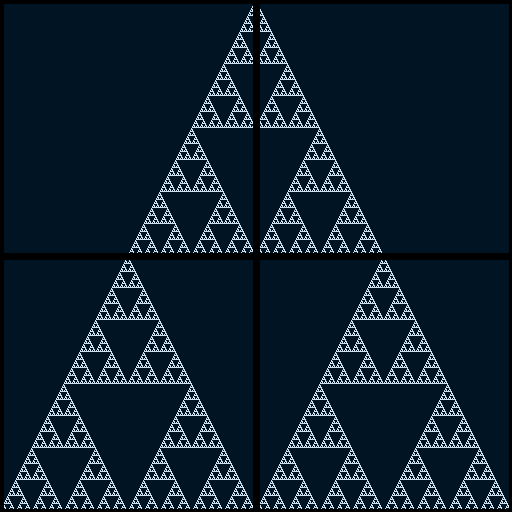
\includegraphics[width=0.5\textwidth]{figures/boxcounting-sierspinsky-1.png}
    \caption{Box Counting - Triángulo de Sierpinski - Cajas de lado $\frac{1}{2}$}
\end{figure}

\noindent Si utilizamos cajas más pequeñas, de lado $\frac{1}{4}$, necesitaremos $12$ cajas.

\begin{figure}[H]
    \centering
    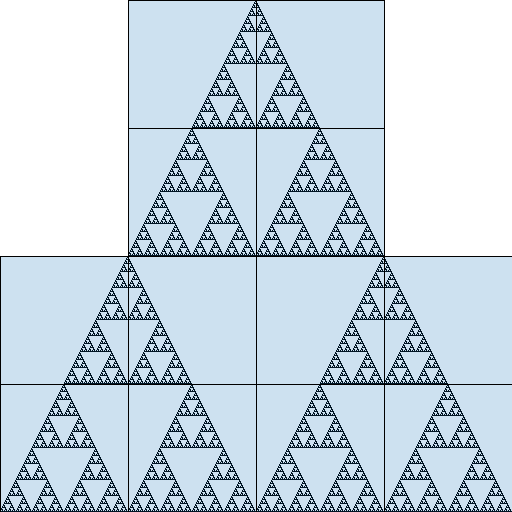
\includegraphics[width=0.5\textwidth]{figures/boxcounting-sierspinsky-2.png}
    \caption{Box Counting - Triángulo de Sierpinski - Cajas de lado $\frac{1}{4}$}
\end{figure}

\noindent Con cajas de lado $\frac{1}{8}$ necesitaremos $36$ cajas.

\begin{figure}[H]
    \centering
    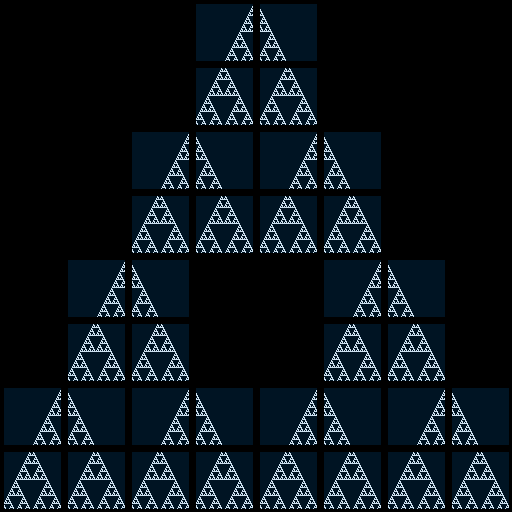
\includegraphics[width=0.5\textwidth]{figures/boxcounting-sierspinsky-3.png}
    \caption{Box Counting - Triángulo de Sierpinski - Cajas de lado $\frac{1}{8}$}
\end{figure}

\noindent Y con cajas de lado $\frac{1}{16}$ necesitaremos $108$ cajas.

\begin{figure}[H]
    \centering
    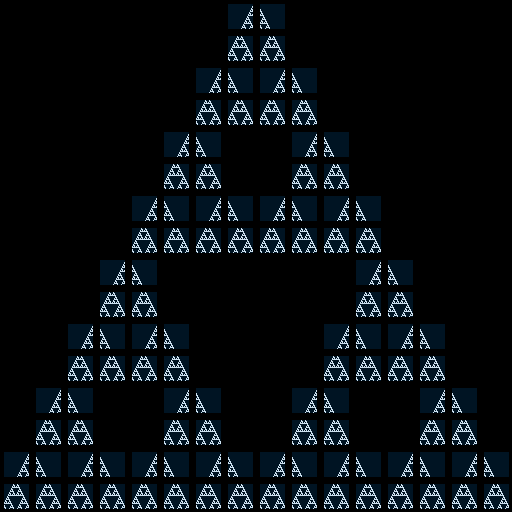
\includegraphics[width=0.5\textwidth]{figures/boxcounting-sierspinsky-4.png}
    \caption{Box Counting - Triángulo de Sierpinski - Cajas de lado $\frac{1}{16}$}
\end{figure}

\noindent Si continuamos con este proceso vemos que para el triángulo de Sierpinski necesitamos $4 \cdot 3^{n-1}$ cajas de lado $\frac{1}{2^n}$.
Si definimos $N(n)$ como el número de cajas de lado $\frac{1}{2^n}$ necesarias para cubrir el objeto, entonces tenemos que:

\begin{equation}
    \begin{split}
        & d = \lim_{n \rightarrow \infty} \frac{log (N(n))}{log (2^n)} = \lim_{n \rightarrow \infty} \frac{4 \cdot 3^{n-1}}{2^n} \approx \\
        & \approx \lim_{n \rightarrow \infty} \frac{3^n}{2^n} = \frac{\log{3}}{\log{2}} \approx 1.585\\
    \end{split}
\end{equation}

\noindent Como ya hemos comentado antes, nos sale un número real. Nuestra intuición nos sugiere que el triángulo de Sierpinski es \textit{"más que una curva"} pero \textit{"menos que una superficie"}\\


\chapter{Historia}

\section{Antecedentes}

\noindent Las primeras formas fractales aparecieron en el siglo XIX, cuando el matemático Karl Weierstrass graficó en 1872 su famosa función de Weierstrass. Más tarde en ese mismo siglo, empezaron a surgir conceptos cada vez más cercanos a lo que hoy se consideran fractales, siendo más gemométricos y menos algebraicos.\cite{complejidad}

\begin{figure}[H]
    \centering
    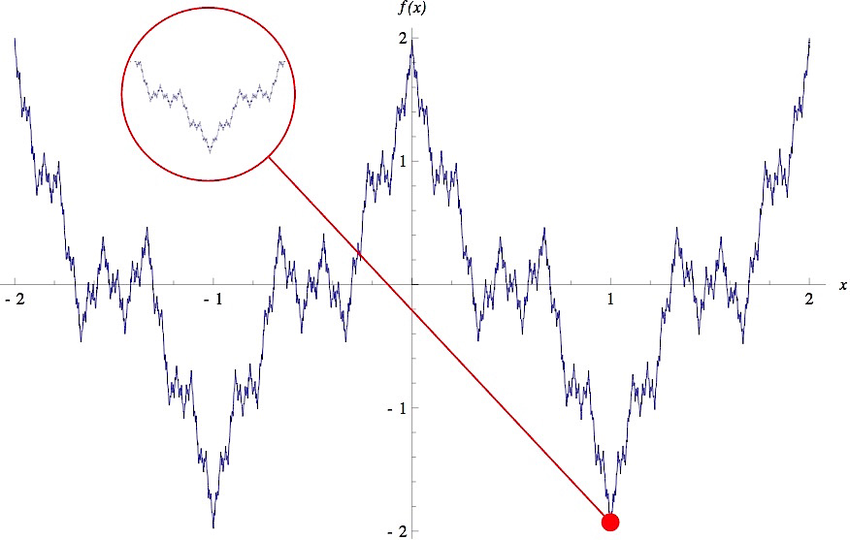
\includegraphics[width=0.5\textwidth]{figures/weierstrass-function.png}
    \caption{Función de Weierstrass}
    \label{fig:weierstrass-function}
\end{figure}

\section{Primeros fractales}

\noindent Así, en 1904, Helge von Koch definió su copo de nieve, una curva con propiedades similares a la de Weierstrass. En 1915, Waclaw Sierspinski construyó su triángulo y, un año después, su alfombra. \cite{complejidad}

\begin{figure}[H]
    \centering
    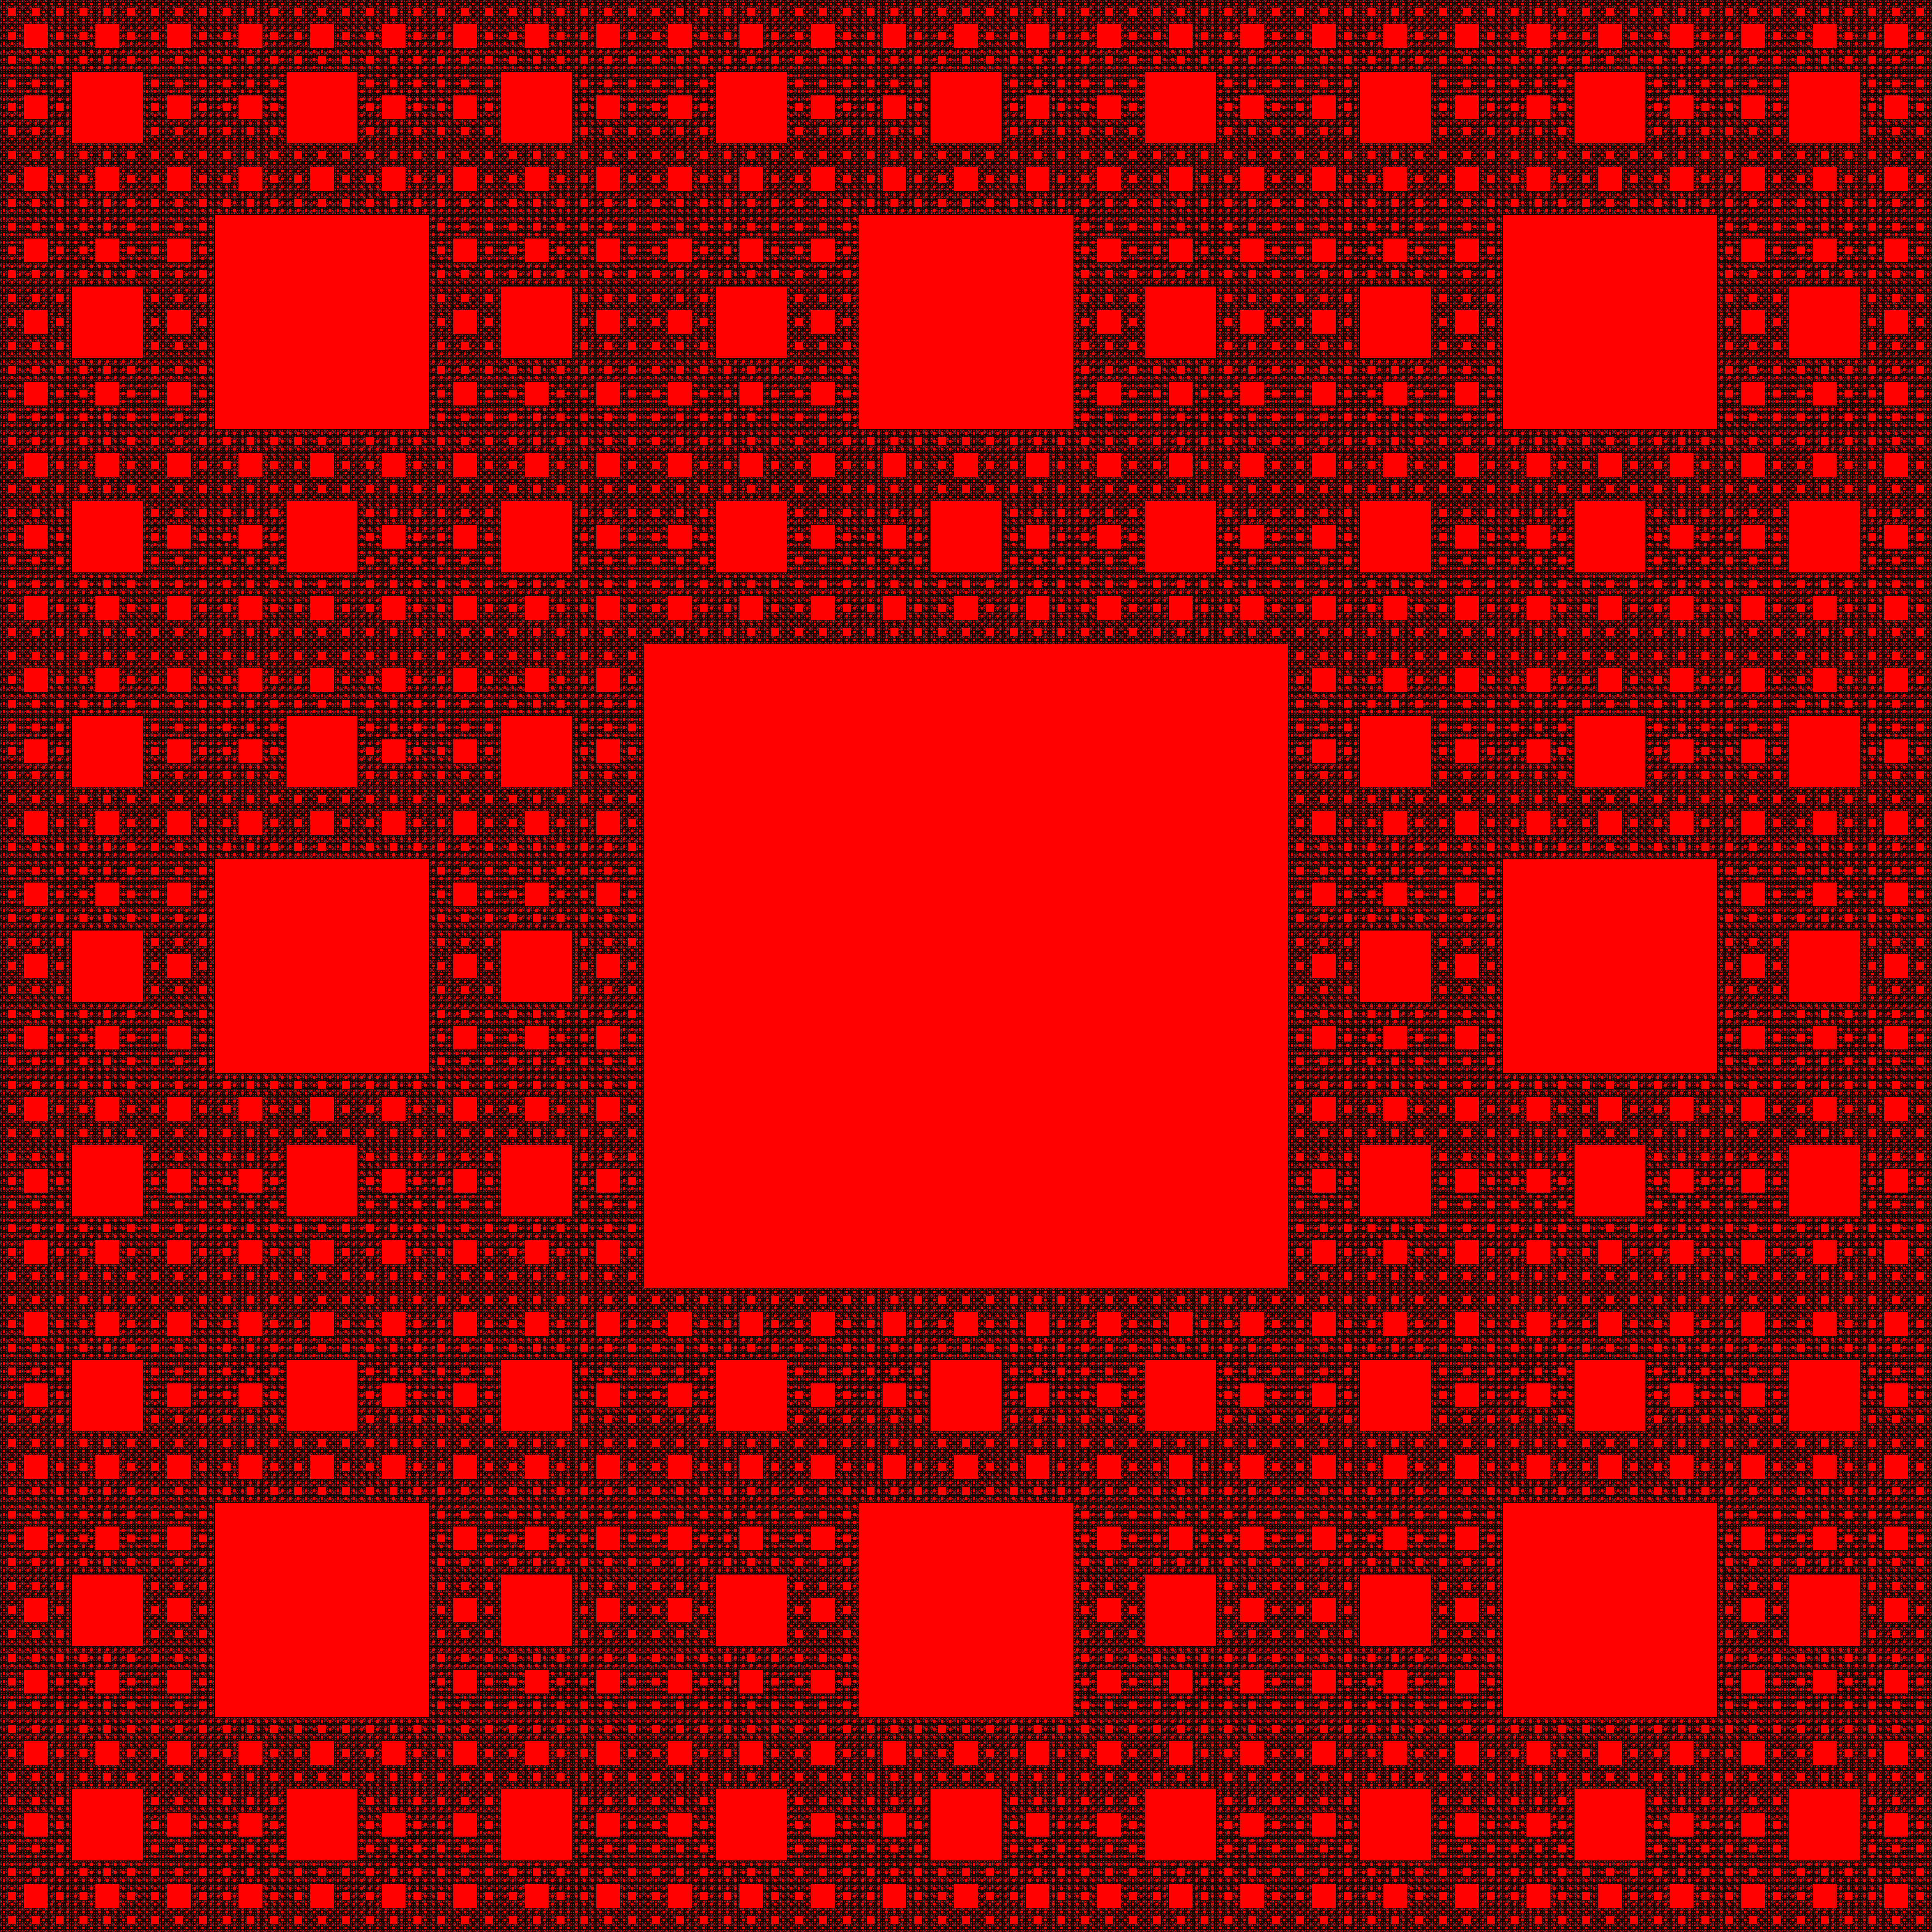
\includegraphics[width=0.5\textwidth]{figures/sierspinsky-carpet.png}
    \caption{Alfombra de Sierspinsky}
    \label{fig:sierspinsky-carpet}
\end{figure}

\section{Nuevas matemáticas}

\noindent En el siglo XIX, Georg Cantor desarrolló su conjunto de Cantor y 
Giuseppe Peano su curva de Peano. Gracias a esto se dieron cuenta de que estos objetos matemáticos no eran casos particulares, si no que había un gran conjunto de funciones que compartían las mismas cualidades que la función de Weierstrass. \cite{complejidad}\\ 

\begin{figure}[H]
    \centering
    
\includegraphics[width=0.5\textwidth]{figures/peano-curve.jpg}
    \caption{Curva de Peano}
    \label{fig:peano-curve}
\end{figure}


\noindent A pesar de que hubiese un gran conjunto de funciones, la geometría de Euclides y la dinámica Newtoniana no podían describirlas bien. En 1919, el matemático Félix Hausdorff introdujo la primera manera de observar y estudiar estos objetos, la dimensión de Hausdorff-Besicovitch. Años más tarde, Andrei Kolmogorov describió una herramienta similar conocida como la entropía de Kolmogorov. \cite{complejidad} \\

\noindent En 1963, Benoît Mandelbrot empezo a trabajar con los fractales a raíz de otra investigación, lo que le llevó a fundar la geometría fractal. \cite{complejidad}

\section{Mandelbrot}

\noindent Mandelbrot es uno de los mayores exponentes en el avance del campo de los fractales, desde identificar una muestra de \textit{"tiempo fractal"} hasta replantearse un problema mundialmente conocido: ¿Cuál es la longitud de la costa de Gran Bretaña? Según Mandelbrot esta distancia es infinita, o mejor dicho, depende de la longitud de la regla con la que se mida. Como ya hemos comentado, la geometría euclídea no es capaz de describir estos objetos, por lo que Mandelbrot utilizó la noción de dimensión, y en concreto, la extraña definición de dimensión fraccionarias. \cite{complejidad}\\

\noindent En 1975, Mandelbrot acuñó el término fractal, que proviene del latín \textit{fractus}, que significa roto o fracturado. El fractal más famoso de Mandelbrot es el conjunto de Mandelbrot, el cual es el más estudiado dentro del campo. \cite{complejidad}

\begin{figure}[H]
    \centering
    
\includegraphics[width=0.5\textwidth]{figures/mandelbrot-set-1.jpg}
    \caption{Conjunto de Mandelbrot}
    \label{fig:mandelbrot-set}
\end{figure}

\appendix

\chapter{Código para la visualización del Box Counting}

\section{Visualización de la recta y el cuadrado}

\begin{lstlisting}[language=Python]
from PIL import Image, ImageDraw

def generar_imagen(n, path):
        
    A = (100,100)
    B = (200,100)
    
    a = (300,100)
    b = (400,100)
    c = (300,200)
    d = (400,200)
        
    img = Image.new('RGB', (500,300), color = 'white')
        
    # Segmento AB
        
    draw = ImageDraw.Draw(img, 'RGBA')
    draw.line((A,B)*100, fill='black', width=1)
        
    # Cuadrado abcd
        
    draw.line((a,b), fill='black', width=1)
    draw.line((b,d), fill='black', width=1)
    draw.line((d,c), fill='black', width=1)
    draw.line((c,a), fill='black', width=1)
    
    # Cajas del segmento AB
    
    for i in range(0,n):
        a = (100+i*(1/n)*100,100+100*1/(2*n))
        b = (100+i*(1/n)*100,100-100*1/(2*n))
        c = (100+(i*100+100)*(1/n),100-100*1/(2*n))
        d = (100+(i*100+100)*(1/n),100+100*1/(2*n))
            
        draw.polygon([a,b,c,d], fill=(0,100,180,50), outline='black', )
        
    # Cajas del cuadrado abcd
        
    for i in range(0,n):
        for k in range(0,n):
            a = (300+k*1/n*100,100+i*1/n*100)
            b = (300+k*1/n*100,100+(i+1)*1/n*100)
            c = (300+(k+1)*1/n*100,100+(i+1)*1/n*100)
            d = (300+(k+1)*1/n*100,100+i*1/n*100)
                
            draw.polygon([a,b,c,d], fill=(0,100,180,50), outline='black')
                
    img.save(path)
        
if __name__ == "__main__":
    N = (2,3,16)
        
    for i in N:
        generar_imagen(i, 'boxcounting-' + str(N.index(i) + 1) + '.png')        
\end{lstlisting}

\section{Visualización del triángulo de Sierpinski}

Créditos a \href{https://github.com/umnikos/Python-Pillow-Library---A-Basic-Example}{umnikos} por el código.

\begin{lstlisting}[language=Python]
from PIL import Image, ImageDraw
import numpy as np
    
size = (512, 512)  # the size of the final image
# create a new black and white image
im = Image.new("1", size, 1)
px = im.load()  # create a pixel access object
    
# takes a 4-tuple range of where to draw the sierpinski triangle
def triangle(xy, fill=0, depth=5):
    # if recursion is over, fill the top left pixel
    if depth == 0:
        px[xy[0], xy[1]] = fill
        return
    # otherwise, draw 3 smaller sierpinski triangles
    triangle(
        (
            (3 * xy[0] + xy[2]) // 4,
            xy[1],
            (xy[0] + 3 * xy[2]) // 4,
            (xy[1] + xy[3]) // 2,
        ),
        fill,
        depth - 1,
    )
    triangle(
        (
            xy[0],
            (xy[1] + xy[3]) // 2,
            (xy[0] + xy[2]) // 2,
            xy[3],
        ),
        fill,
        depth - 1,
    )
    triangle(
        (
            (xy[0] + xy[2]) // 2,
            (xy[1] + xy[3]) // 2,
            xy[2],
            xy[3],
        ),
        fill,
        depth - 1,
    )
    
# draw the triangle (smaller depths results in a dotty output)
triangle((0, 0, size[0], size[1]), depth=10)
            
im.save("sierspinsky.png", "PNG")  # save the image
\end{lstlisting}

\section{Visualización de Box Counting para el triángulo de Sierpinski}

\begin{lstlisting}[language=Python]
import numpy as np
from PIL import Image, ImageDraw

triangle = Image.open('sierspinsky.png')

# Cargar imagen como matriz de pixeles
img_array = np.array(triangle)

def check_pixel_square(top_point, size):
    for i in range(0, size):
        for k in range(0, size):
            if img_array[top_point[1]+ i][top_point[0] + k] == False:
                return True
    return False

def generate_image(n, path):
    img = Image.new('RGB', (512,512), color = 'white')
    img.paste(triangle, (0,0))

    draw = ImageDraw.Draw(img, 'RGBA')

    size = int(512 / n)

    num_cajas = 0

    for i in range(0, n):
        for k in range(0, n):
            if check_pixel_square((i*size,k*size), size):
                draw.rectangle([(i*size,k*size),((i+1)*size,(k+1)*size)], fill=(0,100,180,50), outline='black', width=1)
                num_cajas += 1

    img.save(path)
    print(num_cajas)
    
if __name__ == "__main__":
    
    N = (2,4,8,16)
    
    for i in N:
        generate_image(i, 'boxcounting-sierspinsky-' + str(N.index(i) + 1) + '.png')
\end{lstlisting}

\bibliographystyle{plainurl}
\bibliography{bibliography.bib}


\end{document}